\section{Avoiding Line-Connectivity Constraints\label{sec:app1:lines}}

On line~\ref{alg:app1:tree-Vallow} of Alg.~\ref{alg:app1:tree}, we utilize the expanded potential adjacency matrix ($\xvar{A}$) to disallow connections between components. This is also phrased as every graph must have edges between vertices that are feasible. These are termed vertex-connectivity constraints, denoted \ref{ch2:s5}. A similar type of NSC can be included between the lines of the graph, termed line-connectivity constraints.

\subsection{Theory}

The line graph of a graph \gls{G} is the graph with the edges of $G$ as its vertices, and where two edges of $G$ are adjacent in the line graph if and only if they are incident in $G$ \cite[p.~10]{Godsil2001a}.
Consider the graph in Fig.~\ref{fig:app1:line-connectivity-1} and its corresponding line graph in Fig.~\ref{fig:app1:line-connectivity-2} with three component types.
If component type 1 is connected to component type 2, we can specify if a connection between component types 2 and 3 is allowed. This is equivalent to specifying if line type $(1,2)$ can be connected to line type $(2,3)$.

This enhancement is a new type of NSC and is designated $S_8$.

\begin{figure}[!ht]
\centering
\begin{subfigure}[b]{0.35\textwidth}
\centering

\includegraphics[scale=1]{../app1/fig/line-connectivity-1}
\caption{$G$.\label{fig:app1:line-connectivity-1}}
\end{subfigure}%
\begin{subfigure}[b]{0.35\textwidth}
\centering
 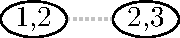
\includegraphics[scale=1]{../app1/fig/line-connectivity-2}
 \caption{Line graph of $G$.\label{fig:app1:line-connectivity-2}}
\end{subfigure}%

\caption{Illustration of a line-connectivity constraint.}
\end{figure}

\subsection{Implementation}

Since this enhancement is a new type of NSC, it is specified before the graph generation procedure. For each line-connectivity constraint, a triple of integers is supplied defining the component types in Fig.~\ref{fig:app1:line-connectivity-1}. They are supplied in increasing order, i.e.,~$[\#1, \#2, \#3]$. Therefore, each triple is interpreted as: 
if \#1 and \#2 are connected, don't ever connect \#2 to \#3.
These triples help construct the reduced 3-D array with line-connectivity constraint information, \gls{B}. They are indexed in reverse order to facilitate extracting column vectors, i.e.,~$B(\#3,\#2,\#1) = 0$.
Given a set of triples, a function creates the expanded $N \times N \times N$ matrix where $N$ is the total number of component replicates where a zero indicates a connection is not allowed and one indicates it is allowed.

\begin{vAlgorithm}[!ht]{\textwidth}{0em}
\LinesNumbered
\DontPrintSemicolon

\SetKwFunction{find}{find}
\SetKwFunction{eye}{eye}
\SetKwFunction{length}{length}

\SetKwInOut{Input}{Input}
\SetKwInOut{Output}{Output}

\caption{Limit potential connections based on line-connectivity constraints.\label{alg:app1:lines}}

\Input{%
        \xvbox{2.5mm}{$\xvar{A}$} -- expanded potential adjacency matrix \\
        \xvbox{2.5mm}{$\xvar{iR}$} -- component index for right port \\
        \xvbox{2.5mm}{$\xvar{iL}$} -- component index for left port \\
        \xvbox{2.5mm}{$\xvar{B}$} -- 3-D array with line-connectivity constraint information \\
      }
\Output{%
        \xvbox{2.5mm}{$\xvar{A}$} -- expanded potential adjacency matrix
       }

\BlankLine

\If{there are any line-connectivity constraints}{

$\xvar{A}(:, \xvar{iR})$ $\leftarrow$ $\xvar{A}(:,\xvar{iR}) \circ \xvar{B}(:,\xvar{iR},\xvar{iL})$ \tcc*{potentially limit connections}

$\xvar{A}(:, \xvar{iL})$ $\leftarrow$ $\xvar{A}(:,\xvar{iL}) \circ \xvar{B}(:,\xvar{iL},\xvar{iR})$ \tcc*{potentially limit connections}

$\xvar{A}([\xvar{iR},\xvar{iL}],:)$ $\leftarrow$ $\xvar{A}(:,[\xvar{iR},\xvar{iL}])\tran$ \tcc*{make symmetric}

}

\end{vAlgorithm}

Algorithm~\ref{alg:app1:lines} is the pseudocode for the implementation of this enhancement.
This enhancement is only called if there are any line-connectivity constraints, $S_8$.
First using the component index of the right port, we extract a vector from the 3-D array with line-connectivity constraint information ($\xvar{B}$) when $\#1 = \xvar{iL}$ and $\#2 = \xvar{iR}$.
This vector is multiplied element-wise with the correct row of the expanded potential adjacency matrix (\xvar{A}), potentially limiting connections.
This step then performed again switching the roles of component indices, i.e.,~$\#1 = \xvar{iR}$ and $\#2 = \xvar{iL}$.
Finally, the changes to $\xvar{A}$ are applied to the symmetric location, ensuring $\xvar{A}$ remains symmetric.

This enhancement is inserted between lines~\ref{alg:app1:tree-A2} and \ref{alg:app1:tree-if} of Alg.~\ref{alg:app1:tree} using the local copy $\xvar{A2}$.

\subsection{Examples}

\subsubsection{Example 1\label{sec:app1:lines-ex1}}

The base three-tuple and NSCs for this example are specified as:
\begin{align}
C = \{ \xcolor{X}, \xcolor{Y}, \xcolor{Z} \}, \quad R = [1\ 2\ 2], \quad P = [2\ 2\ 2], \quad S_8(1) = [1,2,3]
\end{align}

\noindent The reduced ($B$) and expanded ($\xvar{B}$) 3-D arrays with line-connectivity constraint information are:
\vspace{-0.1in}
\begin{align}
B(:,:,1) =
\begin{blockarray}{cccc}
& \xcolor{X} & \xcolor{Y} & \xcolor{Z}  \\
\begin{block}{c[ccc]}
\xcolor{X} & 1 & 1 & 1 \\
\xcolor{Y} & 1 & 1 & 1 \\
\xcolor{Z} & 1 & 0 & 1 \\
\end{block}
\end{blockarray}, \quad 
\xvar{B}(:,:,1) =
\begin{blockarray}{cccccc}
& \xcolor{X} & \xcolor{Y} & \xcolor{Y} & \xcolor{Z} & \xcolor{Z}  \\
\begin{block}{c[ccccc]}
\xcolor{X} & 1 & 1 & 1 & 1 & 1  \\
\xcolor{Y} & 1 & 1 & 1 & 1 & 1  \\
\xcolor{Y} & 1 & 1 & 1 & 1 & 1  \\
\xcolor{Z} & 1 & 0 & 0 & 1 & 1  \\
\xcolor{Z} & 1 & 0 & 0 & 1 & 1  \\
\end{block}
\end{blockarray}
\end{align}
\vspace{-2em}

\noindent Figure~\ref{tb:app1:lines-ex1-V} goes through the operations in Algorithm~\ref{alg:app1:lines} for a certain line type.
The limiting of potential edges is visualized in Fig.~\ref{fig:app1:line-ex1-edge1}.

Table~\ref{tb:app1:lines-ex1} compares the original algorithm with the enhancement for this example. There is a reduction in candidate graphs generated while the number of unique graphs remains the same.

\vspace{-0.1in}

\begin{figure}[!ht]
\centering
\begin{subfigure}[b]{0.4\textwidth}
\centering
\begin{tabular}{r | c }
\hline \hline
& Line Type 1 \\
\hline
\xvar{iL} & 1 \\
\xvar{iR} & 2 \\
$\xvar{B}(:,\xvar{iR},\xvar{iL})$ & $[1\ 1\ 1\ 0\ 0]\tran$ \\
$\xvar{B}(:,\xvar{iL},\xvar{iR})$ & $[1\ 1\ 1\ 1\ 1]\tran$ \\
\hline \hline
\end{tabular}
\caption{Algorithm operations.\label{tb:app1:lines-ex1-V}}
\end{subfigure}%
\begin{subfigure}[b]{0.4\textwidth}
\centering
 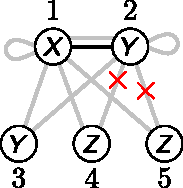
\includegraphics[scale=1]{../app1/fig/line-ex1-edge1_v2}
 \caption{Line Type 1.\label{fig:app1:line-ex1-edge1}}
\end{subfigure}%

\caption{\nameref{sec:app1:lines-ex1} for Algorithm~\ref{alg:app1:lines} (line-connectivity constraints).}
\end{figure}

\begin{table}[!ht]
\centering
\caption{Comparison (line-constraints, \nameref{sec:app1:lines-ex1}).\label{tb:app1:lines-ex1}}
\begin{tabular}{r | c | c | c}
\hline \hline
& Orig & En & Orig/En \\
\hline
Candidate Graphs & 146 & 98 & 1.49 \\
Unique Graphs & 26 & 26 & 1 \\
Generation Time (s) & 0.004 & 0.005 & 0.80 \\
Total Time (s) & 0.036 & 0.034 & 1.06 \\
\hline \hline
\end{tabular}
\end{table}

\subsubsection{Example 2\label{sec:app1:lines-ex2}}

The base three-tuple and NSCs for this example are specified as:
\begin{align}
\begin{gathered}
C = \{ \xcolor{X}, \xcolor{Y}, \xcolor{Z} \}, \quad R = [2\ 2\ 3], \quad P = [2\ 2\ 2] \\
S_8(1) = [1,2,2], \quad S_8(2) = [2,1,2], \quad S_8(3) = [3,3,3]
\end{gathered}
\end{align}

\noindent The reduced 3-D array with line-connectivity constraint information ($B$) is:
\begin{align}
\begin{gathered}
B(:,:,1) =
\begin{blockarray}{cccc}
& \xcolor{X} & \xcolor{Y} & \xcolor{Z}  \\
\begin{block}{c[ccc]}
\xcolor{X} & 1 & 1 & 1 \\
\xcolor{Y} & 1 & 0 & 1 \\
\xcolor{Z} & 1 & 1 & 1 \\
\end{block}
\end{blockarray}, \quad
B(:,:,2) =
\begin{blockarray}{cccc}
& \xcolor{X} & \xcolor{Y} & \xcolor{Z}  \\
\begin{block}{c[ccc]}
\xcolor{X} & 1 & 1 & 1 \\
\xcolor{Y} & 0 & 1 & 1 \\
\xcolor{Z} & 1 & 1 & 1 \\
\end{block}
\end{blockarray} \\ 
B(:,:,3) =
\begin{blockarray}{cccc}
& \xcolor{X} & \xcolor{Y} & \xcolor{Z}  \\
\begin{block}{c[ccc]}
\xcolor{X} & 1 & 1 & 1 \\
\xcolor{Y} & 1 & 1 & 1 \\
\xcolor{Z} & 1 & 1 & 0 \\
\end{block}
\end{blockarray} 
\end{gathered}
\end{align}
\vspace{-2em}

\noindent The expanded 3-D arrays with line-connectivity constraint information ($\xvar{B}$) for $S_8(3)$ are:
\begin{align}
\begin{aligned}
\xvar{B}(:,:,5) = \xvar{B}(:,:,6) = \xvar{B}(:,:,7) =
\begin{blockarray}{cccccccc}
& \xcolor{X} & \xcolor{X} & \xcolor{Y} & \xcolor{Y} & \xcolor{Z} & \xcolor{Z} & \xcolor{Z} \\
\begin{block}{c[ccccccc]}
\xcolor{X} & 1 & 1 & 1 & 1 & 1 & 1 & 1 \\
\xcolor{X} & 1 & 1 & 1 & 1 & 1 & 1 & 1 \\
\xcolor{Y} & 1 & 1 & 1 & 1 & 1 & 1 & 1 \\
\xcolor{Y} & 1 & 1 & 1 & 1 & 1 & 1 & 1 \\
\xcolor{Z} & 1 & 1 & 1 & 1 & 0 & 0 & 0 \\
\xcolor{Z} & 1 & 1 & 1 & 1 & 0 & 0 & 0 \\
\xcolor{Z} & 1 & 1 & 1 & 1 & 0 & 0 & 0 \\
\end{block}
\end{blockarray}
\end{aligned}
\end{align}
\vspace{-2em}

\noindent Figure~\ref{tb:app1:lines-ex2-V} goes through the operations in Algorithm~\ref{alg:app1:lines} for two line types.
The limiting of potential edges is visualized in Figs.~\ref{fig:app1:line-ex2-edge1} and \ref{fig:app1:line-ex2-edge2}.

Table~\ref{tb:app1:lines-ex2} compares the original algorithm with the enhancement for this example. There is a reduction in candidate graphs generated while the number of unique graphs remains the same.

\begin{figure}[!ht]
\centering
\begin{subfigure}[b]{1\textwidth}
\centering
\begin{tabular}{r | c | c }
\hline \hline
& Line Type 1 & Line Type 2 \\
\hline
\xvar{iL} & 1 & 5 \\
\xvar{iR} & 3 & 6 \\
$\xvar{B}(:,\xvar{iR},\xvar{iL})$ & $[1\ 1\ 0\ 0\ 1\ 1\ 1]\tran$ & $[1\ 1\ 1\ 1\ 0\ 0\ 0]\tran$ \\
$\xvar{B}(:,\xvar{iL},\xvar{iR})$ & $[1\ 1\ 0\ 0\ 1\ 1\ 1]\tran$ & $[1\ 1\ 1\ 1\ 0\ 0\ 0]\tran$ \\
\hline \hline
\end{tabular}
\caption{Algorithm operations.\label{tb:app1:lines-ex2-V}}
\end{subfigure}%

\begin{subfigure}[b]{0.4\textwidth}
\centering
 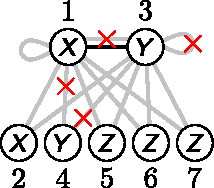
\includegraphics[scale=1]{../app1/fig/line-ex2-edge1_v2}
 \caption{Line Type 1.\label{fig:app1:line-ex2-edge1}}
\end{subfigure}%
\begin{subfigure}[b]{0.4\textwidth}
\centering
 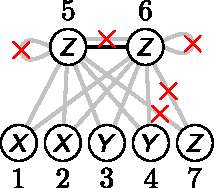
\includegraphics[scale=1]{../app1/fig/line-ex2-edge2_v2}
 \caption{Line Type 2.\label{fig:app1:line-ex2-edge2}}
\end{subfigure}%

\caption{\nameref{sec:app1:lines-ex2} for Algorithm~\ref{alg:app1:lines} (line-connectivity constraints).}
\end{figure}

\begin{table}[!ht]
\centering
\caption{Comparison (line-constraints, \nameref{sec:app1:lines-ex2}).\label{tb:app1:lines-ex2}}
\begin{tabular}{r | c | c | c}
\hline \hline
& Orig & En & Orig/En \\
\hline
Candidate Graphs & 8316 & 5120 & 1.62 \\
Unique Graphs & 119  & 119 & 1 \\
Generation Time (s) & 0.184 & 0.183 & 1.01 \\
Total Time (s) & 2.361 & 2.096 & 1.13 \\
\hline \hline
\end{tabular}
\end{table}